\lab{Algorithm}{Image Segmentation with Minimal Spanning Trees}{Image Segmentation with Minimal Spanning Trees}
\label{Ch:MSTImgSeg}

\objective{This section teaches about how to use minimum spanning trees to segmentate an image.}

\section*{Image Segmentation}

%Lab \ref{MSTImgSeg}

One application of Minimal Spaning Trees (MSTs) is in image segmentation.
Kruskal's algorthm is especially good at this.
Let $k$ be the number of divisions that is wanted and $n$ be the number of nodes.
Kruskals algorithm is performed until $n-k$ edges is added.

There are many different ways to turn a image into a graph and weight the edges.
A simple, yet effective, version is to make every pixel a node and the edges are the difference in intensities in the four cardinal direction. 

This means that there is less that $4n$ edges.
Other image segmentation algorithms have to use $n^2$ space.
This gives the MST algorithm a critical advantage over other image segmentation algorithms. 

\begin{problem}
Write a function that takes as input a black and white image and outputs a list of the edges where thre egdes are in the form $(node,node,weight)$ and a list of nodes.
\end{problem}

The provided kruskal's algorithm takes as inputs the list of nodes, the list of edges and the number of divisions desired.
The number of divisions is often has to be higher than the actual number that is needed because sometimes one or two pixels form a division because the difference between them and the pixels around them is so great.
Adjust the number of divisions until the desired result is found.

\begin{problem}
Perform the image segmentation algorithm on the image.
Then graph the original image and the three highest divisions.
(Use the Counter class from collections to find the modes.) 
\end{problem}

\vfill
\begin{figure}[ht]
\begin{minipage}[b]{0.47\linewidth}
\centering
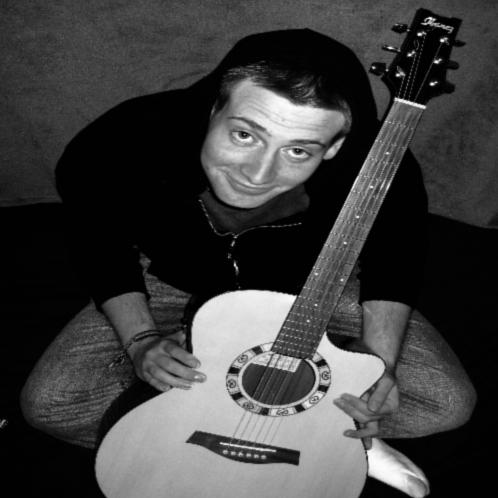
\includegraphics[width=\textwidth]{MSTseg1.jpg}
\end{minipage}
\hspace{0.5cm}
\begin{minipage}[b]{0.47\linewidth}
\centering
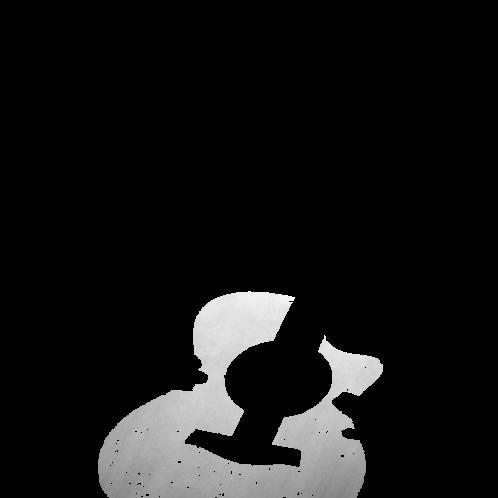
\includegraphics[width=\textwidth]{MSTseg2.jpg}
\end{minipage}
\begin{minipage}[b]{0.47\linewidth}
\centering

\includegraphics[width=\textwidth]{MSTseg3.jpg}
\end{minipage}
\hspace{0.5cm}
\begin{minipage}[b]{0.47\linewidth}
\centering
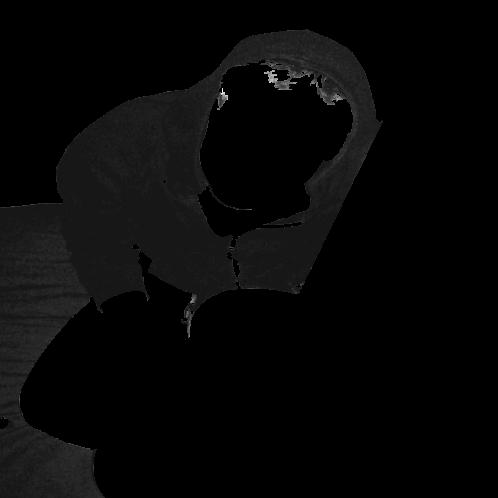
\includegraphics[width=\textwidth]{MSTseg4.jpg}
\end{minipage}
\caption{The original image is in the top left hand corner. The three larges potions are graphed in the other corners. The original image was 498x498 and 50000 divisions were used. TODO get permission to use this picture}
\end{figure}
\vfill

\begin{problem}
Make a division of the image a different color.
\end{problem}

This algorithm can also be extended to 3D images.
One configuration is that each pixel is a node and the edges are the four cardinal directions, the pixel directly above it and the pixel below it.

This algorithm can also be used to segment other data such as connections on facebook. 
